\documentclass{article}
\usepackage[british]{babel}
\usepackage{times}
\usepackage{amsmath}
\usepackage{mathtools}
\usepackage{amsfonts}
\usepackage{verbatim}
\usepackage{lmodern}
\usepackage{tikz}
\usepackage[ruled,vlined]{algorithm2e}
\usetikzlibrary{patterns}

\numberwithin{equation}{section}

\newtheorem{lemma}{Lemma}[section]

\DeclareMathOperator*{\argmax}{arg\,max}
\DeclareMathOperator*{\argmin}{arg\,min}

\DeclareMathOperator*{\KL}{{\rm KL}}

\setlength{\parskip}{1em}

\begin{document}

\title{Bayesian averaging for variational inference applied to genomic data - First Draft}
\author{William van Rooij - EPFL}

\maketitle

\newpage
\tableofcontents
\newpage
\section{Introduction}
For the past years, data science has been increasingly present in the world. From financial establishments to road management companies, a lot of industry sectors are integrating data science in the way business is done. With the expansion of computer performance, we are able to implement faster computation and can work with more complex models. The volume of available data, hence analysable data, is also growing, which allows more accurate inference.

Often, when trying to find a model fitting the observable data, we have much more observations than parameters to fit. We work in a \textit{large n - small p} situation. It is the most common type of statistical analysis, Bayesian hierarchical modelling is a strong tool to identify the dependencies across multiple sources of informations. However, in some cases, the number of parameters to estimate is much larger than the number of observations available. It is often the case in genomic research, where the situation is called a \textit{small n - large p}. Traditional techniques do not apply in these environment, because of both statistical and computational constraints.

In this report, we will focus on the \textit{small n - large p} situation in the context of genetic association. We will focus on high dimensional Bayesian inference, with its statistical advantages and its computational problem that often dissuades users to adopt this solution in statistical applications.

\subsection{Motivation}
The state of the technology nowadays allows us to determine the human genome. With this possibility, a whole new set of data is available to study the association between these data and various diseases or phenotypes.  Part of these newly available data are \textit{genetic variants}, a change at a specific location on  the genome (locus), where the different versions are called \textit{alleles}. We will focus on the most common genetic variant, the \textit{single nucleotide polymorphisms} (SNPs), a variation in the nucleotide that is present to some appreciable extent in the population, \textit{i.e.} the \textit{minor} allele has frequency $> 0.01$ \cite{lewin}. Some combinations of SNPs are inherited together, which yields block-wise dependences structures. We observe strong autocorrelations in these blocks, as shows Figure \ref{fig:corr}.
\begin{figure}
\centering
\includegraphics[width=3in,bb = 0 0 2in 1in]{images/CorrSingleNoProba.png}
\caption{\label{fig:corr} Visualisation of the block-wise correlation structure in the SNPs.}
\end{figure}

We focus on \textit{expression quantitative trait locus} (eQTL) analyses, which study the effects of genetic variants, in our case SNPs, on the expression of transcripts, or genes. The data used for eQTL studies consists generally of several hundreds thousands SNPs and thousand transcripts expression outcomes. It is, in fact, a \textit{small n - large p - large q} situation, where $p$ is the number of SNPs and $q$ is the number of transcripts expressions outcomes.

In a Bayesian framework, one of the main tools used are integrals. However, the integrals are usually not amenable and need to be approximated. Markov Chain Monte Carlo (MCMC) algorithms are the standard to estimate these integrals and can be reasonably fast and accurate when working on reasonably small datasets. When the dataset dimensions grow, however, MCMC algorithms become very time-consuming up to not being computable.

When performing MCMC inference, likelihoods and sometimes gradients need to be calculated at each iterations. The cost of these calculations increases with the number of parameters. Moreover, the more dimensions the problem has, the less accurate the approximations become, which leads to more iterations to keep the precision needed. For the algorithm to end, all the parameters need to have converged, which means all parameters need to be checked and stored, which is often impossible when their number is very high.

In our situation, \textit{small n - large p - large q}, the computational cost of using an MCMC algorithm is huge. The time and memory needed to run the algorithm is not acceptable as of today. We have to use an alternative solution, which we choose to be variational inference \cite{varInf}.
%==========================================
\newpage
\section{Model}
We denote $\boldsymbol{X }= (X_1,\ldots,X_p)$ the SNPs and $\boldsymbol{y} = (y_1,\ldots,y_q)$ the traits. The SNPs have strong local correlations structures on the genome. Our goal is to estimate the association between a SNP $s$ and a transcript expression, called \textit{trait}, $t$. To do so, we consider $\boldsymbol{y}$ as the response matrix and $\boldsymbol{X}$ as the candidate predictors of the linear model, where each response $y_t$ is linearly related with the predictors $\boldsymbol{X}$ and has a residual precision $\boldsymbol{\tau}_t$, \textit{i.e.}
\begin{equation*}
\label{eq:model}
\boldsymbol{y}_{n\times q} = \boldsymbol{X}_{n \times p}\;\boldsymbol{\beta}_{p \times q}+\boldsymbol{\epsilon}_{n \times q}\text{, }\boldsymbol{\epsilon}_t \sim \mathcal{N}(0,\tau_t^{-1}I_n),
\end{equation*}
where $\boldsymbol{\beta}_{st}$ represent the association between SNP $s$ and trait $t$. The parameters $\tau_t$ and $\sigma^{-2}$ have the following prior distribution:
\begin{align*}
\tau_t &\sim \text{Gamma}(\eta_t,\kappa_t),\\
\sigma^{-2} &\sim \text{Gamma}(\lambda,\nu).
\end{align*}

We introduce $\boldsymbol{\gamma}_{p\times q}$, a binary matrix which pairs of SNPs - trait are associated. The SNP $s$ and trait $t$ are associated if and only if $\gamma_{st} = 1$. To enforce sparsity in $\boldsymbol{\beta}$, we set a "spike-and-slab" prior distribution on $/beta_{st}$, \textit{i.e.} 
\begin{equation*}
\beta_{st} \mid \gamma_{st},\sigma^2, \tau_t \sim \gamma_{st}\;\mathcal{N}(0,\sigma^2\tau_t^{-1})+(1-\gamma_{st})\;\delta_0
\end{equation*}
where $\delta_0$ is a Dirac distribution.

We call $\omega_s$ the parameter controlling to the proportion of responses associated with the predictor $X_s$. Then, the prior distribution of $\gamma_{st}$ knowing $\omega_s$ is given by:
\begin{equation*}
\gamma_{st} \mid \omega_s \sim  \text{Bernoulli}(\omega_s).
\end{equation*}
We choose $\omega_s$ to follow a Beta distribution,
\begin{equation*}
\omega_s \sim \text{Beta}(a_s, b_s).
\end{equation*}
The parameters $a_s$ and $b_s$ are chosen to enforce sparsity. If we define $p^* \ll p$ as the expected number of predictors involved in the model, we want to set $a_s$ and $b_s$ such that the prior probability that $X_s$ is associated with at least one response is equal to $p^*/p$. We fix the mean of the distribution but let the variance free, the solution still has one degree of freedom so multiple solutions are possible, \textit{e.g.}
\begin{equation*}
a_s \equiv 1,\;b_s \equiv q(p-p^*)/p^*.
\end{equation*}
% =========================================
\newpage
\section{Variational inference}
When computing the posterior density of parameters $\boldsymbol{\theta}$ according to observed data $\boldsymbol{y}$, variational inference simplifies the computation by approximating the posterior density $p(\boldsymbol{\theta}\mid \boldsymbol{y})$ with a simpler density $q(\boldsymbol{\theta})$. It gives an approximation of the posterior distribution as a result of an optimization problem that minimizes a measure of "closeness" as objective function.

Suppose that we have observations $\boldsymbol{y}$ and parameters $\boldsymbol{\theta}$, we need to determine the posterior distribution of the parameters conditional on the observations $p(\boldsymbol{\theta} \mid \boldsymbol{y})$. Given a family of densities $\mathcal{D}$ over the parameters, we want to find the distribution $q \in \mathcal{D}$ that minimizes the "closeness" measure compared to $p(\boldsymbol{\theta} \mid \boldsymbol{y})$.

Variational inference minimizes the Kullback--Leibler divergence as a "closeness" measure. Introduced in 1951 by Kullback and Leibler\cite{kl51}, it is the most common divergence measure used in statistics and machine learning:
\begin{equation*}
\KL(q\parallel p) := \int q(\boldsymbol{\theta})\log \left(\frac{q(\boldsymbol{\theta})}{p(\boldsymbol{\theta} \mid \boldsymbol{y})}\right) \mathrm{d}\boldsymbol{\theta}.
\end{equation*} 
It is described as a "directed divergence" as it is asymmetric, \textit{i.e.}, $\KL(p\parallel q) \neq \KL(q \parallel p)$.

Determining the family $\mathcal{D}$ can be difficult as we need the family to be simple enough to be optimized efficiently, but flexible enough for the approximation $q \in \mathcal{D}$ to be close to $p(\boldsymbol{\theta} \mid \boldsymbol{y})$ with respect to the Kullbach--Leibler divergence. The approximation will then be:
\begin{equation*}
q^*(\boldsymbol{\theta} ) = \argmin_{q(\boldsymbol{\theta}) \in \mathcal{D}} \KL\left( q(\boldsymbol{\theta}) \parallel p(\boldsymbol{\theta} \mid \boldsymbol{y})\right).
\end{equation*}

Minimizing the Kullbach--Leibler divergence can be complicated depending on the density $p$ that we want to approximate and the densities family $\mathcal{D}$ that we want $q$ to be part of. We can decompose the Kullbach--Leibler divergence as follows:
\begin{align*}
\KL\left(q(\boldsymbol{\theta})||p(\boldsymbol{\theta}\mid \boldsymbol{y})\right) &= \mathbb{E}\left[\log q(\boldsymbol{\theta})\right] - \mathbb{E}\left[\log p(\boldsymbol{\theta}\mid \boldsymbol{y})\right]\\
&= \mathbb{E}\left[\log q(\boldsymbol{\theta})\right] - \mathbb{E}\left[\log p(\boldsymbol{y},\boldsymbol{\theta})\right] + \log p(\boldsymbol{y}).
\end{align*}
We introduce the evidence lower bound:
\begin{align*}
\mathcal{L}(q) &= \mathbb{E}\left[\log p(\boldsymbol{\theta},\boldsymbol{y})\right] - \mathbb{E}\left[\log q(\boldsymbol{\theta})\right]\\
&=\int q(\boldsymbol{\theta})\log\frac{p(\boldsymbol{y},\boldsymbol{\theta})}{q(\boldsymbol{\theta})}\mathrm{d}\boldsymbol{\theta}.
\end{align*}
When decomposing the Kullbach--Leibler divergence, we obtain:
\begin{equation*}
\KL(q\parallel p) = \log(p) - \mathcal{L}(q).
\end{equation*}
This means that the Kullbach--Leibler divergence is the difference between the marginal log-likelihood with no effect on the optimization and a function : $\mathcal{L}(q)$. Hence, minimizing the Kullbach--Leibler divergence is the same as maximizing $\mathcal{L}(q)$. The difference lays in the complexity of the problems, minimizing the Kullbach--Leibler divergence is not tractable, but maximizing $\mathcal{L}(q)$ admits a closed form when the family of densities $\mathcal{D}$ is well chosen. In such a case, we prefer to use $\mathcal{L}(q)$ as an objective function.

Jensen's inequality provides another way to see that $\mathcal{L}(q)$ is a lower bound for the marginal log-likelihood, which is why we call it the evidence lower bound, or variational lower bound.
\begin{align*}
\log p(\boldsymbol{y}) &= \log \int p(\boldsymbol{y}, \boldsymbol{\theta}) \mathrm{d}\boldsymbol{\theta},\\
&= \log \int \frac{p(\boldsymbol{y}, \boldsymbol{\theta})}{q(\boldsymbol{\theta})}q(\boldsymbol{\theta})\mathrm{d}\boldsymbol{\theta}
,\\
&\geq \int q(\boldsymbol{\theta}) \log \left\lbrace \frac{p(\boldsymbol{y}, \boldsymbol{\theta})}{q(\boldsymbol{\theta})} \right\rbrace \mathrm{d}\boldsymbol{\theta},\\
&= \mathcal{L}(q).
\end{align*}
Hence, $\log p(\boldsymbol{y}) \geq \mathcal{L}(q)$, justifying the lower bound for $\mathcal{L}(q)$.

\subsection{Mean-field approximation}
The complexity of the optimization problem is directly bound to the complexity of the family of densities $\mathcal{D}$ we want $q(\boldsymbol{\theta})$ to be part of. We introduce the mean-field variational family, where the parameters are mutually independent and are governed by a distinct factor in the variational density.

Let $\left\lbrace \theta_j\right\rbrace_{j=1}^J$ be a partition of $\boldsymbol{\theta}$, if $q \in \mathcal{D}$ and $\mathcal{D}$ is a mean-field variational family, then:
\begin{equation*}
q(\boldsymbol{\theta}) = \prod_{j=1}^J q_j(\theta_j)
\end{equation*}
We determine the variational factors $q_j(\theta_j)$ by maximizing $\mathcal{L}(q_j)$. Hence, the variational family does not directly represent the observed data, they are both linked through the optimization of the evidence lower bound.

Concretely, we assume the independence of most of the parameters:
\begin{equation*}
q(\boldsymbol{\theta}) =\left\lbrace\prod_{s=1}^p \prod_{t=1}^q q(\beta_{st}, \gamma_{st})\right\rbrace \left\lbrace\prod_{s=1}^p  q(\omega_s)\right\rbrace \left\lbrace\prod_{t=1}^q q(\tau_t)\right\rbrace q(\sigma^{-2}).
\end{equation*}

To visualise the mean-field approximation, we consider a two dimensional Gaussian distribution, represented in clear in Figure \ref{fig:mean_field}. The mean-field approximation of the posterior distribution is represented by the barred circle. We can see that the mean of the approximation is the same as the real mean, but the covariance does not match the covariance of the real posterior.

\begin{figure}[h!]
\centering
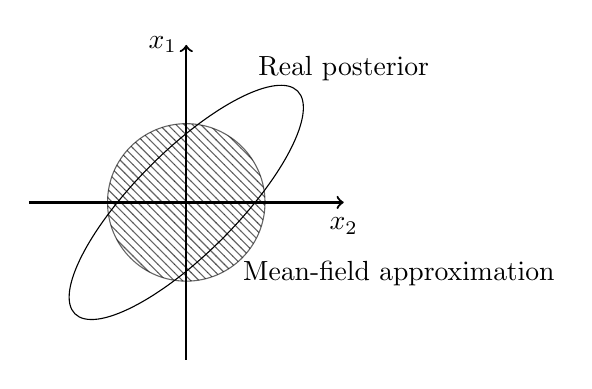
\begin{tikzpicture}
\draw[thick, ->] (0,-2) -- (0,2);
\draw[thick, ->] (-2,0) -- (2,0);
\fill[pattern=north west lines,opacity=.6,draw] (0,0) circle (1cm);
\draw[rotate=-45] (0,0) ellipse (0.65cm and 2cm);
\node (p) at (2,1.7) {Real posterior};
\node (q) at (2.7,-0.9) {Mean-field approximation};
\node (x1) at (-0.3,2) {$x_1$};
\node (x2) at (2,-0.3) {$x_2$};
\end{tikzpicture}
\caption{\label{fig:mean_field}Visualisation of mean-field approximation to a two-dimensional Gaussian posterior. The correlations in the mean-field approximation do not represent the correlations of the real posterior.}
\end{figure}

We have transformed, using the evidence lower bound and the mean-field approximation our problem into a optimization problem. We now need a way to solve this problem. In the following section, we describe the coordinate ascend algorithm.
% =========================================
\subsection{Coordinate ascent algorithm}
The coordinate ascent mean-field variational inference  is one of the most commonly used to solve this type of optimization problem. The algorithm iterates on the parameters of the mean-field approximation, optimizing them one at the time. It yields a local optimum for the evidence lower bound. The algorithm is based on the following result:
\begin{lemma}

If we fix $q_l(\theta_l)$, $l\neq j$, then the optimal $q^*_j(\theta_j)$ verifies:
\begin{equation*}
q^*_j(\theta_j) \propto \exp\left\lbrace\mathbb{E}_{-j}\left[\log p(\theta_j \mid \boldsymbol{\theta}_{-j}, \boldsymbol{y})\right]\right\rbrace.
\end{equation*}
Where $/mathbb{E}_{-j}$ denotes the expectation with respect to all $l \neq j$.
\end{lemma}

Based on this result, the algorithm updates one parameter $\theta_j$ at the time while the others stay fixed. The algorithm stops when $\mathcal{L}(q)$ varies less than a determined threshold $\varepsilon$.

\begin{algorithm}
\SetKwData{ELBO}{$\mathcal{L}(q)$}\SetKwData{OLDELBO}{$\mathcal{L}^{\text{old}}(q)$}
\SetKwFunction{Union}{Union}\SetKwFunction{FindCompress}{FindCompress}
\SetKwInOut{Input}{input}\SetKwInOut{Output}{output}\SetKwInOut{Init}{initialize}
\SetKw{Set}{set}
\Input{$p(\boldsymbol{y},\boldsymbol{\theta})$, dataset $y$ tolerance $\varepsilon$}
\BlankLine
\Output{$q(\boldsymbol{\theta}) = \prod_{j=1}^J q_j(\theta_j)$}
\BlankLine
\Init{$q_j(\theta_j)$}
\BlankLine
\Repeat{$|\mathcal{L}^{\text{old}}(q)-\mathcal{L}(q)| < \varepsilon$}{
\For{$j\in \left\lbrace 1, \ldots, J \right\rbrace $}{\label{forins}
\Set{$q_j(\theta_j) \propto \exp\left\lbrace\mathbb{E}_{-j}\left[\log p(\theta_j \mid \boldsymbol{\theta}_{-j}, \boldsymbol{y})\right]\right\rbrace$}}
\BlankLine
\OLDELBO$\leftarrow$\ELBO\;
\ELBO$\leftarrow\mathbb{E}\left[\log p(\boldsymbol{\theta}, \boldsymbol{y})\right]-\mathbb{E}\left[\log q(\boldsymbol{\theta})\right]$
\BlankLine
}
\Return{$q(\boldsymbol{\theta})$}
\caption{Coordinate ascent variational inference \label{algo:CAVI}}
\end{algorithm}
At every iteration, $\mathcal{L}(q)$ is guaranteed to increase. The algorithm yields a local optimum depending on the initialization of the $q_j(\theta_j)$, $j=1,\ldots,J$. Having different initializations could yield different optima that correspond to different models.

In our case, the posterior distributions of our model's parameters are:
\begin{align*}
\beta_{st} \mid \gamma_{st} = 1, \boldsymbol{y} &\sim \mathcal{N}\left(\mu_{\beta, st},\sigma^2_{\beta, st}\right),\\
\beta_{st} \mid \gamma_{st} = 0, \boldsymbol{y} &\sim \delta_0,\\
\gamma_{st} \mid \boldsymbol{y} &\sim \text{Bernoulli}(\gamma_{st}^{(1)}),\\
\omega_s\mid\boldsymbol{y} &\sim \text{Beta}(a_s^*,b_s^*),\\
\tau_t\mid \boldsymbol{y} &\sim \text{Gamma}(\eta^*_t, \kappa^*_t),\\
\sigma^{-2} \mid \boldsymbol{y} &\sim \text{Gamma}(\lambda^*, \nu^*).
\end{align*}

\newpage
\section{Multimodality}

Bayesian model averaging is a strategy to account for multiple competing models in an inference problem. It consists of weighting the different models in a weighted average with the probability that the data corresponds to each model. The more the model corresponds to the observed data, the more it will stand out in the result.

Assume that the data $\boldsymbol{y}$ correspond to multiple models $M_k$, $k= 1,\ldots,K$, and $\Delta$ is the quantity of interest. We have the posterior distribution:
\begin{equation}
p(\Delta \mid \boldsymbol{y}) = \sum_{k=1}^K p(\Delta \mid M_k,\boldsymbol{y}) \; p(M_k \mid \boldsymbol{y}).
\label{eq:post_dist}
\end{equation}
This corresponds to a weighted average of the posterior distribution under each of the considered models with weights corresponding to the posterior models probabilities.

Instead of $p(\Delta \mid \boldsymbol{y})$ in Equation \ref{eq:post_dist}, we might be interested in approximating:
\begin{equation*}
\mathbb{E}\left[\Delta \mid \boldsymbol{y}\right] = \sum_{k=1}^K\mathbb{E}\left[\Delta \mid M_k, \boldsymbol{y}\right]\;p(M_k \mid \boldsymbol{y}).
\end{equation*}

The posterior probability for model $M_k$ is given by:
\begin{equation}
p(M_k \mid \boldsymbol{y}) = \frac{p(\boldsymbol{y} \mid M_k)\; p(M_k)}{\sum_{j=1}^K p(\boldsymbol{y} \mid M_j)\; p(M_j)},
\label{eq:post_prob}
\end{equation}
where $p(\boldsymbol{y} \mid M_k)$ is the likelihood of model $M_k$, and $p(M_k)$ is the prior probabilities of the model $M_k$. It can, for example, depend on the complexity of the model, to favour the simpler models, or, if we consider the models to be equiprobable, it would be equal to $p(M_k) = 1/K$, $k = 1,\ldots,K$.  

We know that the evidence lower bound and the Kullbach--Leibler divergence are related and that minimizing the Kullbach--Leibler divergence is equivalent to maximizing the evidence lower bound, and that they verify: 
\begin{equation*}
\KL(q\parallel p) = \log p (\boldsymbol{y}) - \mathcal{L}(q).
\end{equation*}
Since we minimized the Kullbach--Leibler divergence, we can use $\mathcal{L}(q)$ as an approximation for $\log p(\boldsymbol{y})$ in Equation \ref{eq:post_prob}.

Our quantity of interest is $\gamma_{st}$, \textit{i.e.} we want to know if the SNP $s$ and the trait $t$ are associated. Using Algorithm \ref{algo:CAVI}, we initialise the distributions $q_j(\theta_j)$ with different starting points, and consider the optimums yielded by the algorithm.

We can consider each optimum to be a model representing the data, and we can apply a form of Bayesian model averaging to combine them all using the method we described here above. We approximate $\log p(\boldsymbol{y})$ by $\mathcal{L}(q)$ in Equation \ref{eq:post_prob}, and obtain an approximation for $\mathbb{E}\left[\gamma_{st}\mid \boldsymbol{y}\right]$ considering all the models we have obtained in the algorithm.
% =========================================
\newpage
\section{Simulations}
In her R-package \texttt{locus}, H. Ruffieux has implemented a function \texttt{locus} that estimates the probabilities of association between a SNP and a trait. We will use this function to build our own method and also to have a comparison. If our method would not perform better than this implementation, it because irrelevant.

Our method is basically calling multiple times that \texttt{locus} function and combine all the results in an weighted average. For each call, we initialized the parameters differently, and hoped to obtain different optimums.

We have drawn at random the initial parameters for the optimal approximations $q^*(\boldsymbol{\theta})$. We have used H. Ruffieux's function \texttt{locus} to calculate the probabilities of association between the SNPs and the traits, as well as the evidence lower bound for each initialisation. Then we used the evidence lower bounds as weights in our variant of Bayesian model averaging to combine the results of each initialisation.

We first tested our method on generated data, to be able to compare the results calculated with the truth. We have used H. Ruffieux's R-package \texttt{echoseq} to generate block wise strongly autocorrelated SNPs and traits, as well as their associations. We have generated $300$ observations of $500$ SNPs, with autocorrelations between $0.95$ and $0.99$, by blocks of $10$ SNPs. As we want to visualise the probabilities of association, we generated just one trait. We did $100$ random initialisations for the parameters.

In Figure \ref{fig:ROCComp}, we have plotted the ROC curves of our method (blue) as well as the ROC curve of calling the function just once (orange). We replicated the process $50$ times to generate these curves, so we don't get "lucky" and have the a set of parameters that is really performing well and would not be representative of the real behaviour of the method. We have chosen the number of SNPs associated with the trait to be $15$ or $50$, and the maximum proportion of response variance explained by the SNPs to be $0.5$ or $0.8$.
\begin{figure}[h!]
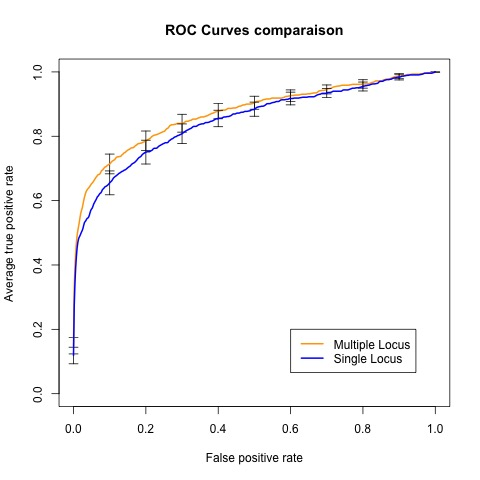
\includegraphics[width=2.7in, bb= 0 0 1.7in 1.7in]{images/ROC_Comp_p0_15_var_0_5.jpeg}
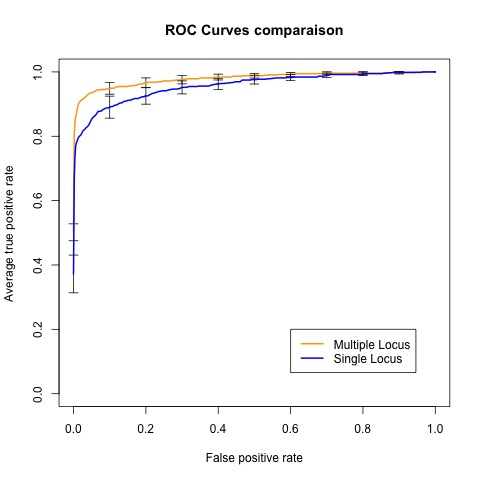
\includegraphics[width=2.7in, bb= 0 0 1.7in 1.7in]{images/ROC_Comp_p0_15_var_0_8.jpeg}
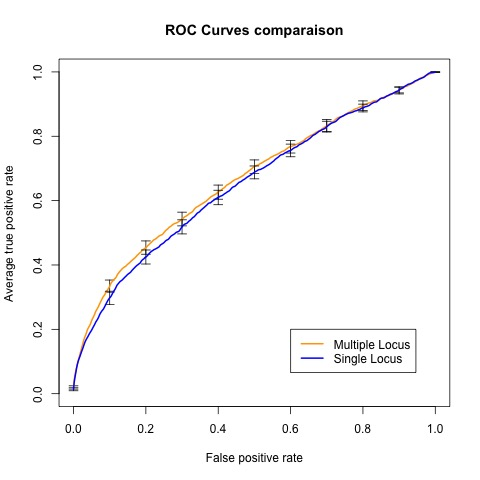
\includegraphics[width=2.7in, bb= 0 0 1.7in 1.7in]{images/ROC_Comp_p0_50_var_0_5.jpeg}
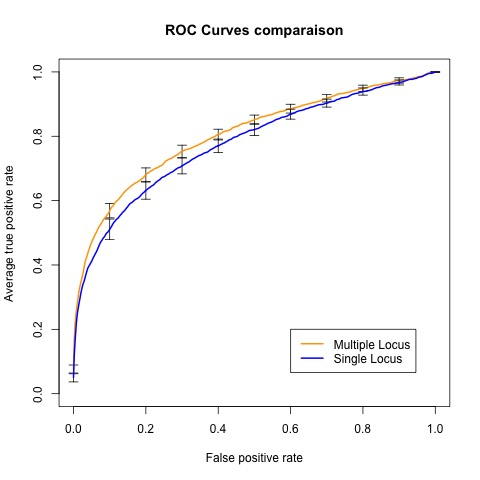
\includegraphics[width=2.7in, bb= 0 0 1.7in 1.7in]{images/ROC_Comp_p0_50_var_0_8.jpeg}
\caption{\label{fig:ROCComp}Comparison of ROC curves between single locus (blue) and multiple locus (orange). Top: $p_0 = 15$, Left: Max tot. PVE$ = 0.5$,
Bottom: $p_0 = 50$, Right: Max tot. PVE$ = 0.8$}
\end{figure}

We can see that with every parameters combination, our method performs better than the single-call method. We can see that some combinations of parameters yield better results than others. For example, we can see that when the maximum proportion of response variance explained by the SNPs is bigger, the method identifies better the SNPs associated with the trait (right two compared to left two). In the same way, the method identifies better the active SNPs when their number is lower (top two compared to bottom two).


It should be noted that for our method, paralleled computation is possible, which can drastically diminish the time needed to compute it. Even if the method has to wait until the last iteration to converge, we would still be quicker than calculating the iterations one after the other.
% =========================================
\newpage
\section{Next steps}
For the remainder of this project, we will compare the accuracy of our approach and its computational cost to other methods, such as annealing and non-weighted averaging for strong correlations. We will also try to combine annealing with our method.\cite{glob}

To be able to tell if our algorithm adequatly explores the local modes, we will represent them with the level curves similarly as V. Rockova \cite{rockova} did.

We plan to optimize the code that we implemented, to have an acceptable comparison with the other methods commonly used. If the results are satisfactory, we may include the function in H. Ruffieux's R-package (http://github.com/hruffieux/locus).

Finally, to be able to apply this method on real-life data would be the target of the whole project.
\newpage
\bibliography{references}
\bibliographystyle{plain}
\end{document}